\section{Phương pháp đề xuất}
\subsection{Kiến trúc dữ liệu lớn}

Google Cloud cung cấp một loạt các dịch vụ và công cụ mạnh mẽ để xây dựng và quản lý kiến trúc dữ liệu lớn. Các dịch vụ này giúp doanh nghiệp thu thập, lưu trữ, xử lý và phân tích dữ liệu một cách hiệu quả. Một số dịch vụ chính của Google Cloud trong kiến trúc dữ liệu lớn bao gồm:

\begin{itemize}
    \item \textbf{Google Cloud Storage}: Dịch vụ lưu trữ đối tượng có khả năng mở rộng cao, cho phép lưu trữ và truy cập dữ liệu không giới hạn.
    \item \textbf{Google Cloud Dataflow}: Một dịch vụ xử lý dữ liệu theo lô và theo luồng, hỗ trợ các mô hình lập trình như Apache Beam.
\end{itemize}
Với các dịch vụ này, Google Cloud giúp doanh nghiệp xây dựng các giải pháp dữ liệu lớn linh hoạt, hiệu quả và dễ dàng mở rộng, từ đó tối ưu hóa quá trình ra quyết định dựa trên dữ liệu.

\textbf{Ingest: Google Cloud Storage}
\begin{figure}[H]
    \centering
    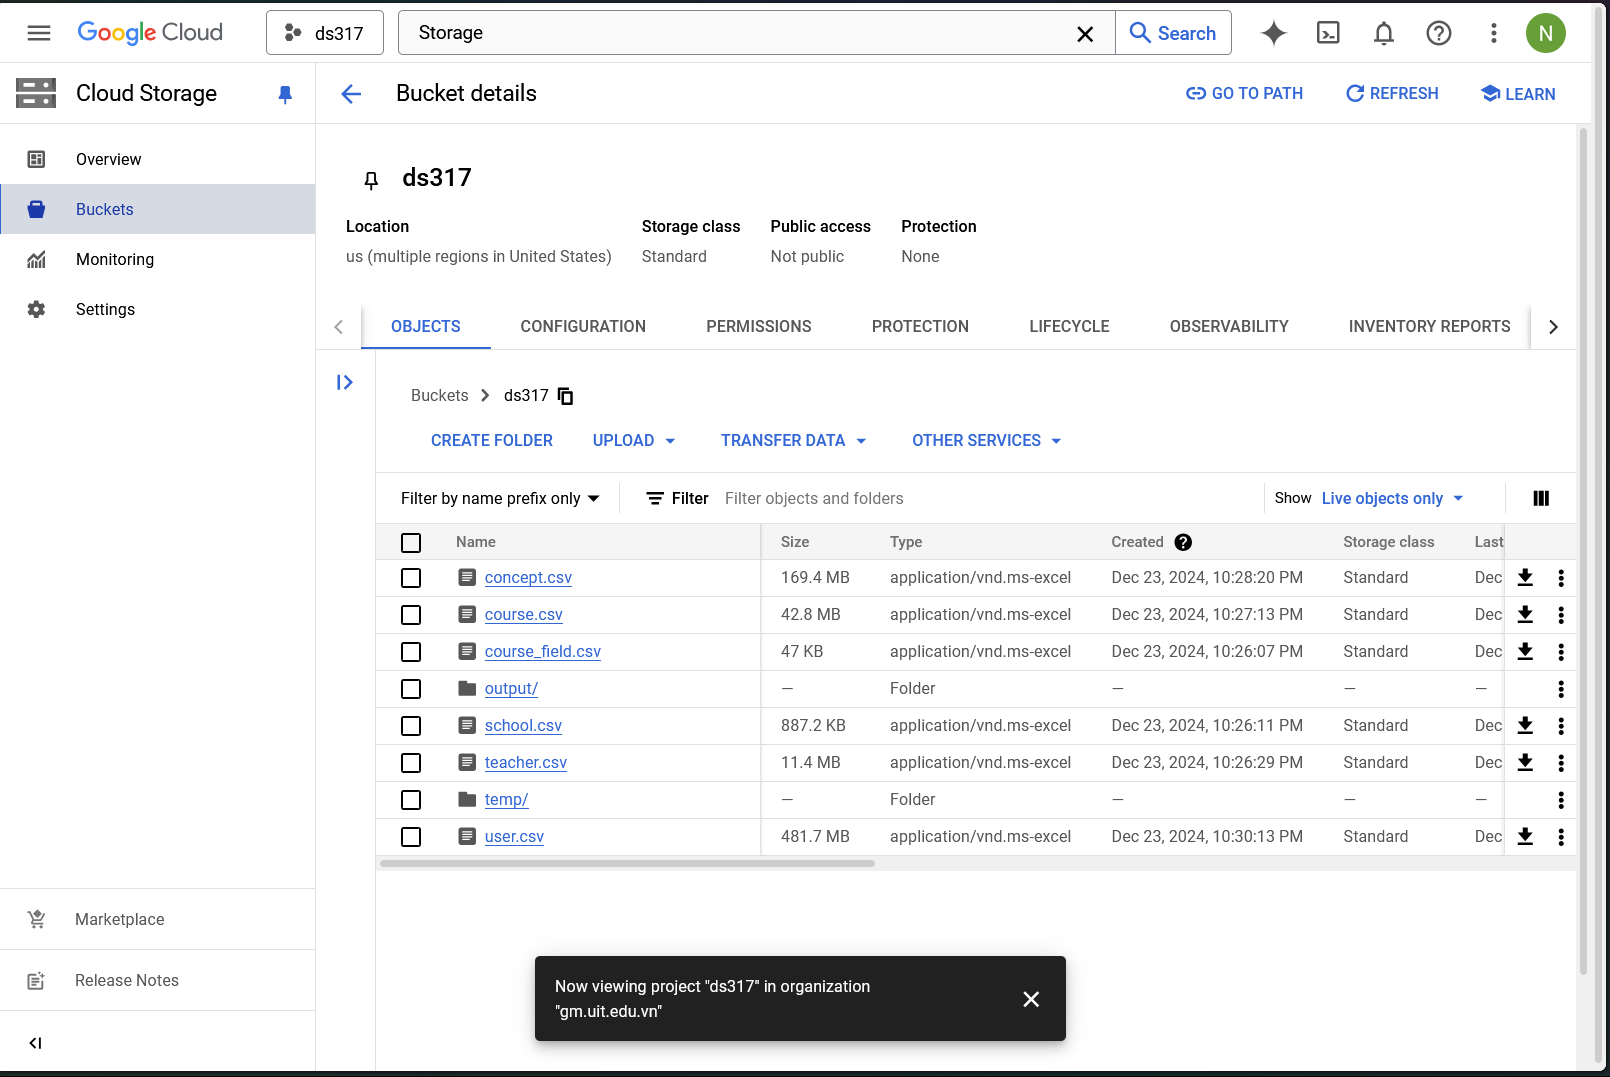
\includegraphics[width=0.8\textwidth]{figures/73.png}
    \caption{Hình ảnh lưu trữ dữ liệu thu thập từ MOOCCubeX}
\end{figure}

\textbf{Process: Google Cloud Dataflow}
\begin{figure}[H]
    \centering
    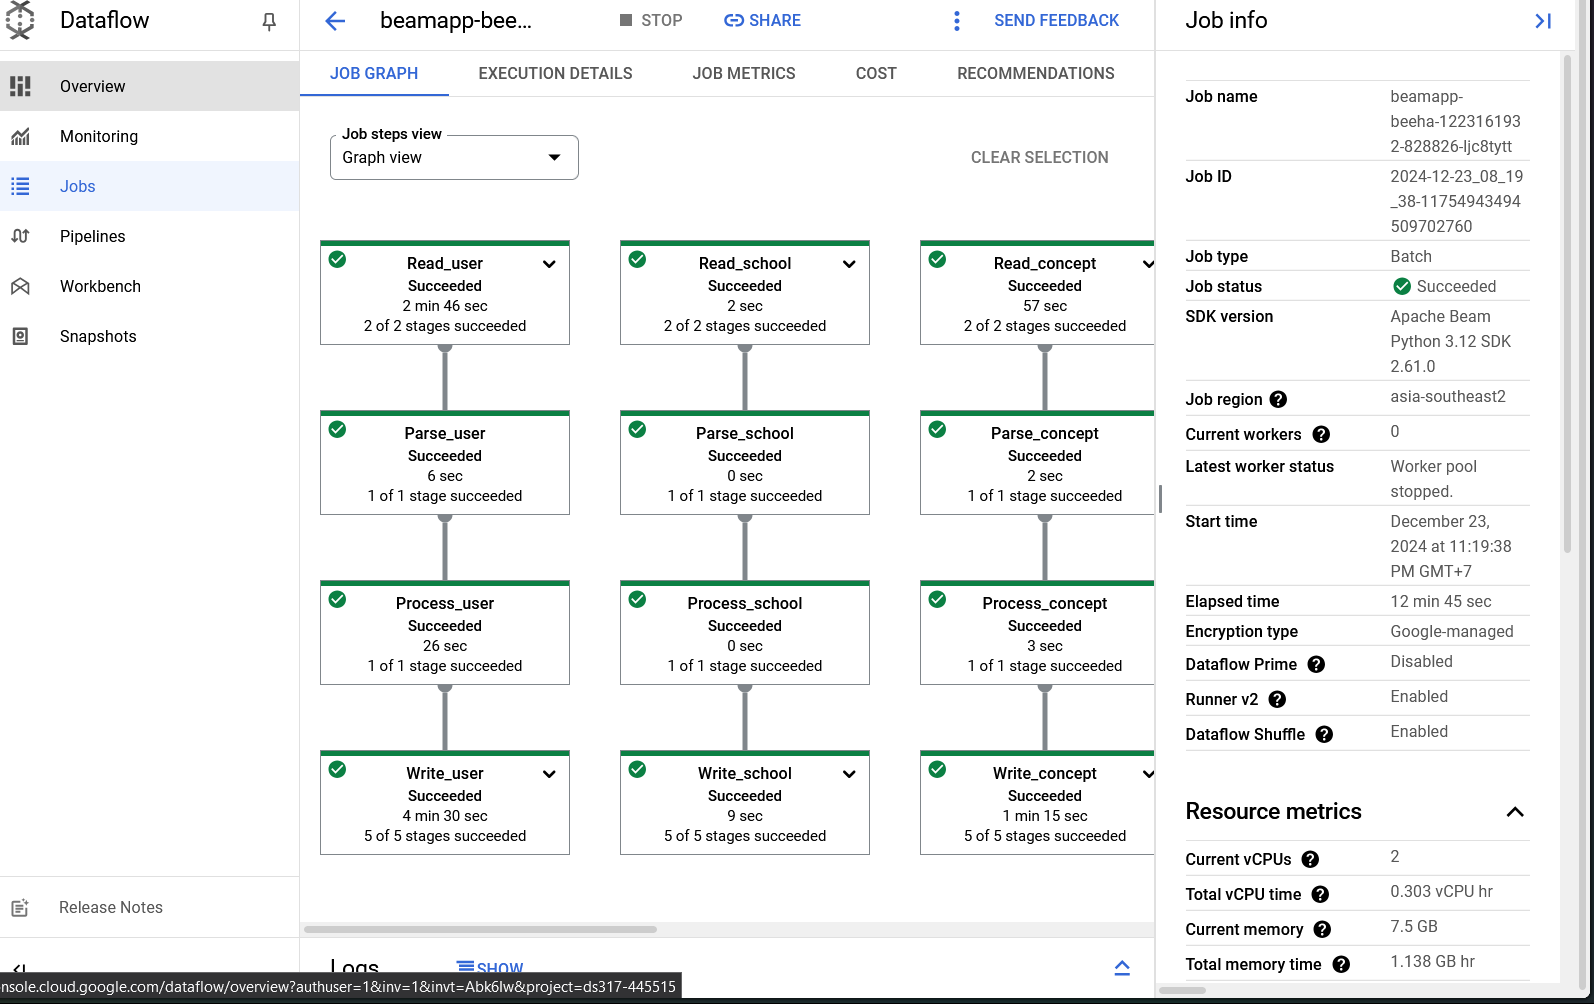
\includegraphics[width=0.8\textwidth]{figures/74.png}
    \caption{Hình ảnh xử lý dữ liệu từ MOOCCubeX}
\end{figure}
\subsection{Ứng dụng web}
\subsubsection{Flask}

Flask là một framework phát triển web nhẹ, đơn giản và dễ sử dụng trong Python.
Được tạo ra bởi Armin Ronacher, Flask thuộc dạng "micro-framework", nghĩa là nó
không đi kèm với quá nhiều tính năng mặc định, cho phép lập trình viên tự do lựa
chọn và tích hợp các thành phần mà họ cần. Đặc điểm chính của Flask:
\begin{itemize}
    \item Nhẹ nhàng và dễ mở rộng: Flask chỉ cung cấp những tính năng cơ bản như
        định tuyến URL, quản lý yêu cầu và phản hồi HTTP. Các tính năng nâng cao như cơ sở dữ liệu, xác thực hay quản lý phiên người dùng có thể được thêm qua các thư viện mở rộng.
    \item Dễ học và sử dụng: Flask được thiết kế với cú pháp đơn giản, dễ đọc,
        phù hợp cho cả người mới học lập trình web và các chuyên gia phát triển.
    \item Không gò bó: Không giống như các framework lớn như Django, Flask không
        ép buộc bạn phải tuân theo một kiến trúc cụ thể. Bạn có thể tự do tổ chức dự án theo cách riêng của mình.
\end{itemize}

\subsubsection{PostgreSQL}

PostgreSQL (thường được gọi là Postgres) là một hệ quản trị cơ sở dữ liệu quan
hệ mã nguồn mở mạnh mẽ và linh hoạt. Được phát triển từ năm 1986 tại Đại học
California, Berkeley, Postgres đã trở thành một trong những hệ thống cơ sở dữ
liệu phổ biến và được tin cậy nhất hiện nay. Đặc điểm nổi bật của PostgreSQL:
\begin{itemize}
    \item Hệ quản trị cơ sở dữ liệu quan hệ đối tượng (ORDBMS): PostgreSQL hỗ
        trợ không chỉ dữ liệu quan hệ truyền thống mà còn có khả năng lưu trữ và xử lý dữ liệu dạng đối tượng, JSON, XML, và các loại dữ liệu không gian (spatial data).

    \item Mã nguồn mở và miễn phí: PostgreSQL là một dự án mã nguồn mở, nghĩa
        là bạn có thể sử dụng, chỉnh sửa và phân phối mà không mất phí. Nhiều công ty lớn sử dụng Postgres làm nền tảng cơ sở dữ liệu của họ.

    \item Hiệu suất cao: PostgreSQL được tối ưu hóa để xử lý khối lượng lớn dữ
        liệu và thực hiện các truy vấn phức tạp một cách hiệu quả.

    \item Hỗ trợ đa nền tảng: PostgreSQL có thể chạy trên nhiều hệ điều hành
        như Linux, Windows, macOS, và các hệ thống UNIX khác.

    \item Cộng đồng lớn: PostgreSQL có một cộng đồng phát triển và người dùng
        đông đảo, cung cấp tài liệu, hỗ trợ kỹ thuật và nhiều tiện ích mở rộng.
\end{itemize}

\subsubsection{Thiết kế cơ sở dữ liệu}

Dữ liệu của MOOCCubeX được lưu trữ dưới các file json và txt, vì vậy nhóm cần
phải chuyển các file này vào cơ sở dữ liệu của PostgreSQL. Trước hết, nhóm cần phải
thiết kế một lược đồ cơ sở dữ liệu để lưu trữ các thông tin cần thiết cho việc demo:

\begin{figure}[H]
    \centering
    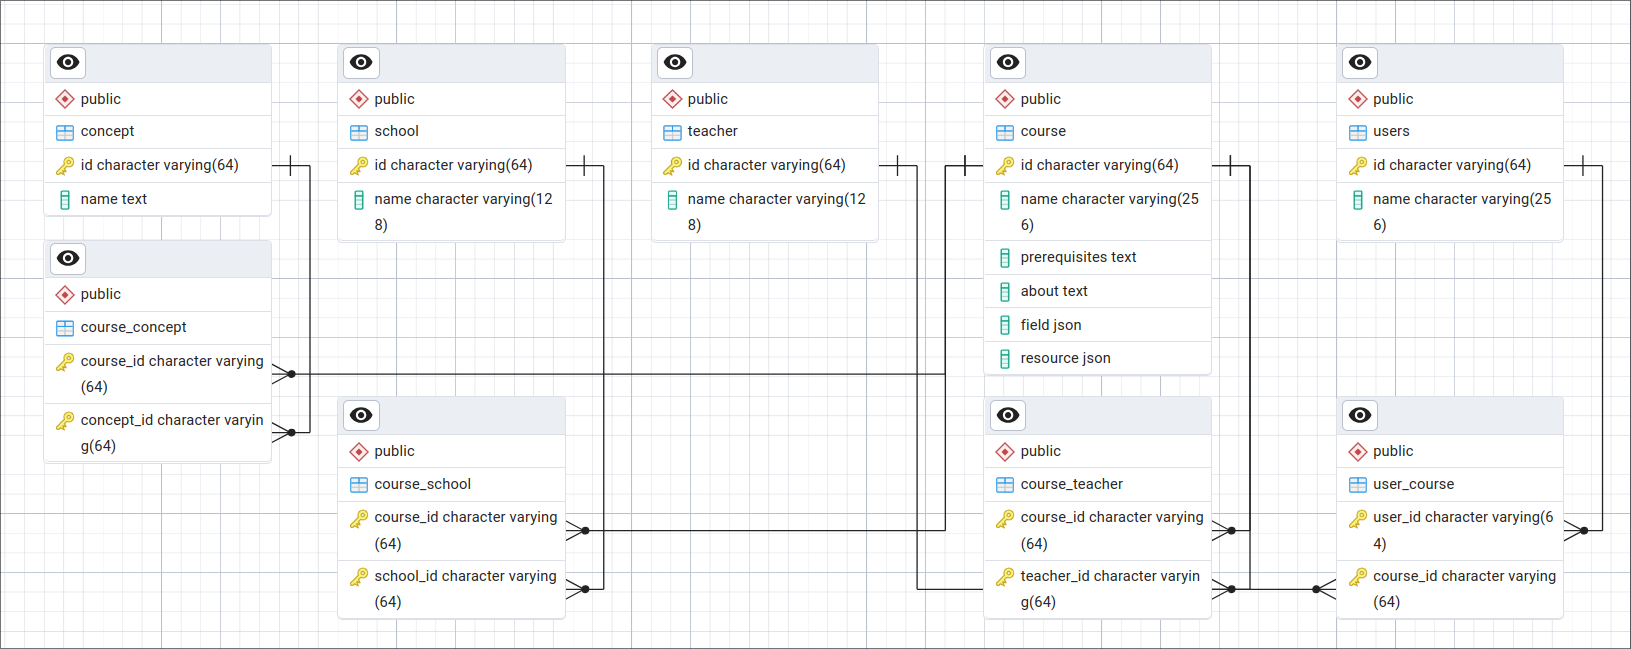
\includegraphics[width=0.8\textwidth]{figures/72.png}
    \caption{Cơ sở dữ liệu}
\end{figure}

\subsubsection{Thiết kế giao diện}

React là một thư viện JavaScript mạnh mẽ được sử dụng để xây dựng các giao diện người dùng tương tác và hiệu quả. Với khả năng tái sử dụng các thành phần (components) và quản lý trạng thái (state) một cách linh hoạt, React giúp các nhà phát triển dễ dàng tạo ra các ứng dụng web phức tạp và có hiệu suất cao.

Trong dự án này, chúng tôi sử dụng React để xây dựng giao diện người dùng cho hệ thống quản lý khóa học. Giao diện này bao gồm các tính năng chính như tìm kiếm khóa học, xem thông tin chi tiết về khóa học, và khuyến nghị các khóa học phù hợp với người dùng. Dưới đây là một số chi tiết về thiết kế giao diện:

\begin{itemize}
    \item \textbf{Trang chủ}: Trang chủ cung cấp một cái nhìn tổng quan về các khóa học phổ biến và mới nhất. Người dùng có thể dễ dàng tìm kiếm các khóa học thông qua thanh tìm kiếm hoặc duyệt qua các danh mục khóa học.
    \item \textbf{Tìm kiếm khóa học}: Tính năng tìm kiếm cho phép người dùng nhập từ khóa và nhận được danh sách các khóa học liên quan. Kết quả tìm kiếm được hiển thị một cách rõ ràng và có thể lọc theo các tiêu chí như lĩnh vực, cấp độ, và đánh giá.
    \item \textbf{Thông tin khóa học}: Khi người dùng chọn một khóa học, họ sẽ được chuyển đến trang chi tiết khóa học. Trang này cung cấp thông tin chi tiết về khóa học bao gồm mô tả, nội dung, giảng viên, và đánh giá từ các học viên khác.
    \item \textbf{Khuyến nghị khóa học}: Dựa trên hành vi và sở thích của người dùng, hệ thống sẽ khuyến nghị các khóa học phù hợp. Tính năng này giúp người dùng dễ dàng tìm thấy các khóa học mà họ có thể quan tâm.
    \item \textbf{Quản lý tài khoản}: Người dùng có thể đăng nhập và họ cũng có thể xem lịch sử học tập và tiến trình của mình.
\end{itemize}

\begin{figure}[H]
    \centering
    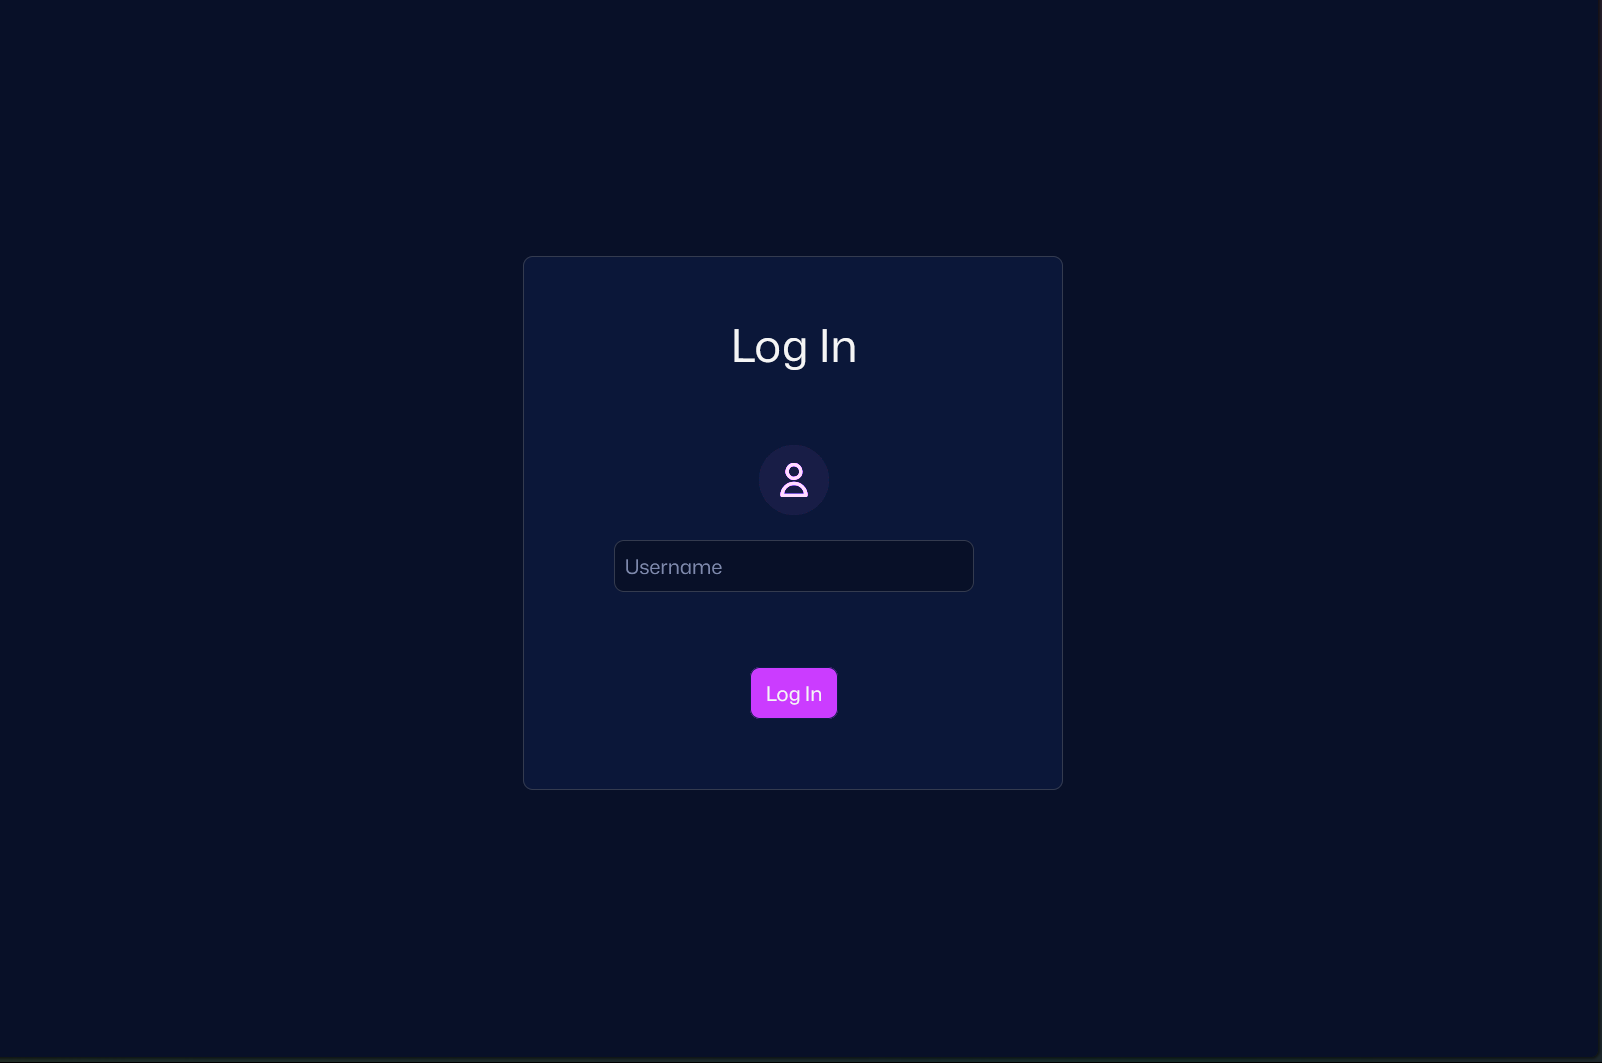
\includegraphics[width=0.8\textwidth]{figures/75.png}
    \caption{Trang login}
\end{figure}

\begin{figure}[H]
    \centering
    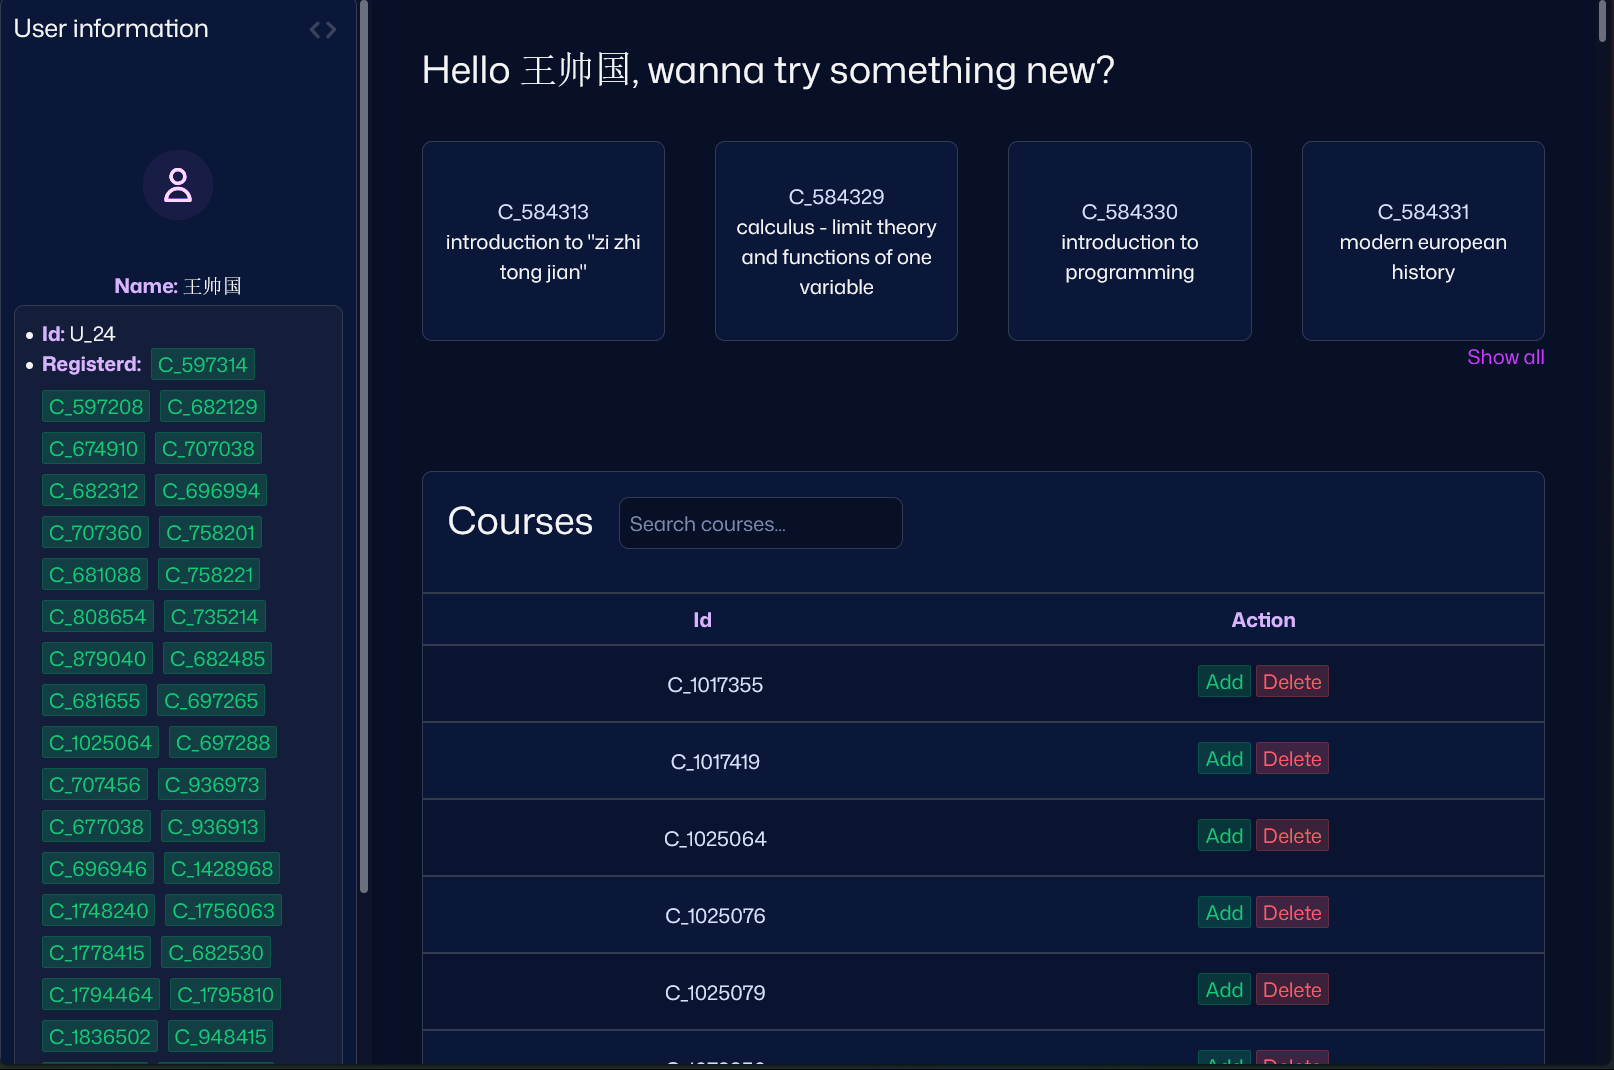
\includegraphics[width=0.8\textwidth]{figures/76.png}
    \caption{Trang chủ: Gồm thông tin tài khoản, khoá học khuyến nghị và tất cả khoá học}
\end{figure}

\begin{figure}[H]
    \centering
    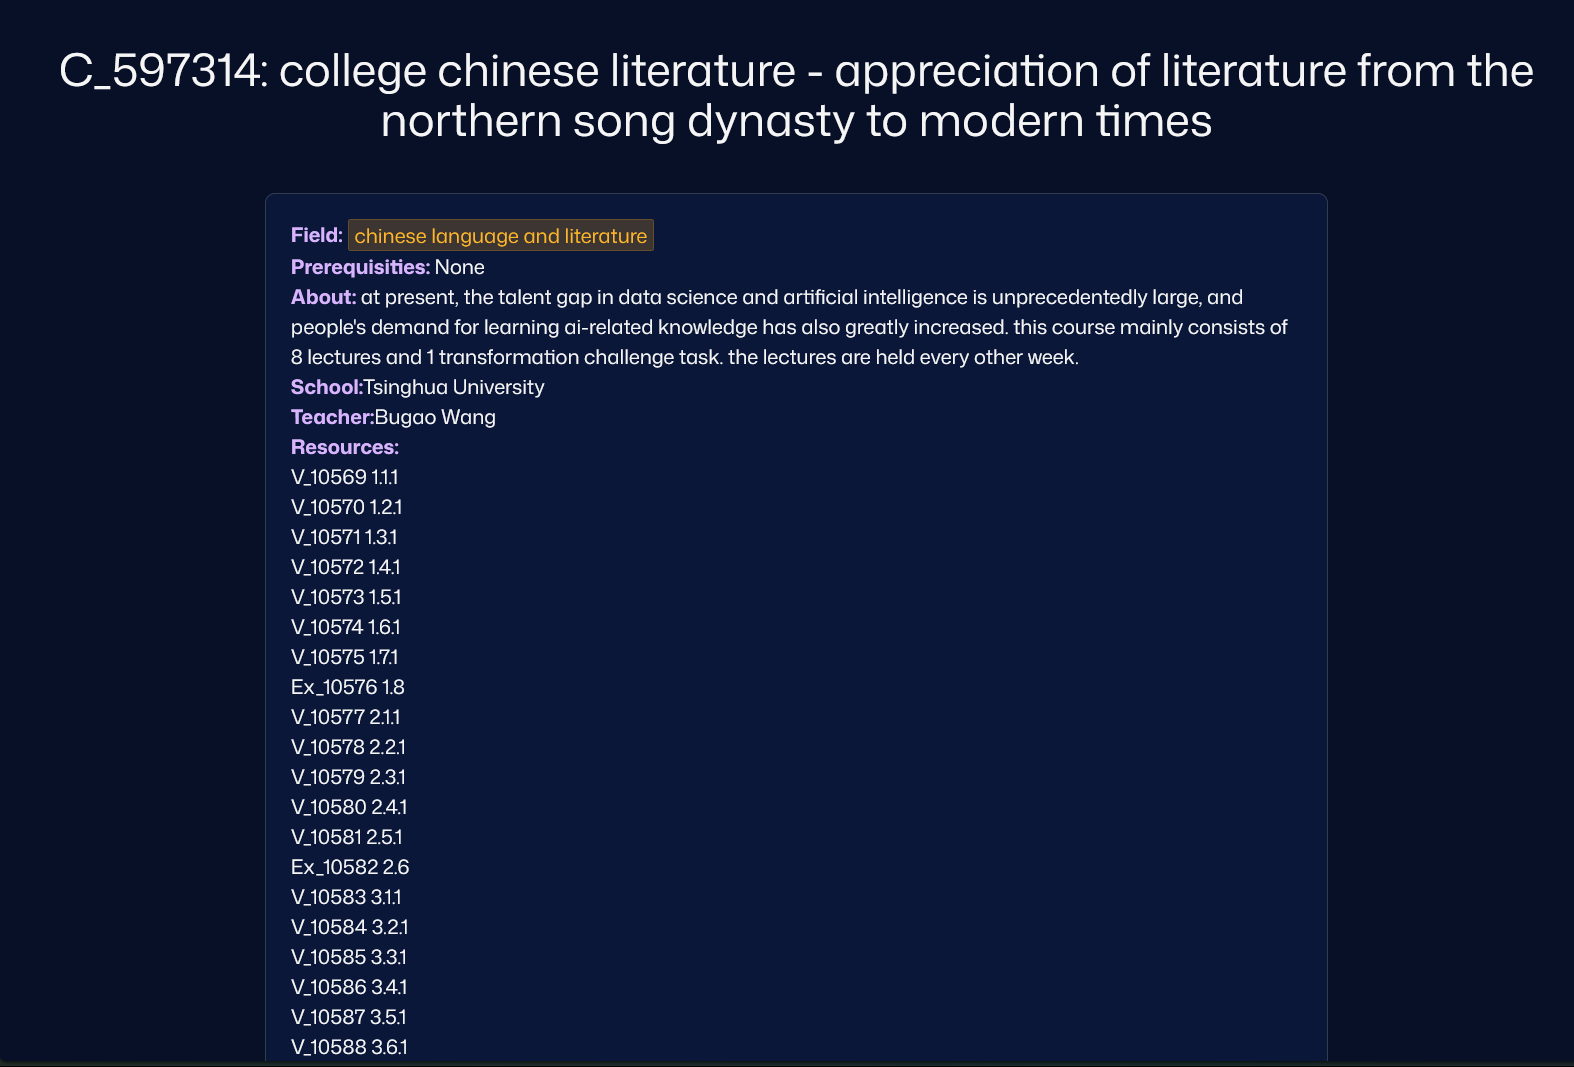
\includegraphics[width=0.8\textwidth]{figures/77.png}
    \caption{Trang chi tiết khoá học}
\end{figure}